\documentclass[beamer=true]{standalone}
\usepackage{preamblesnotes}

\begin{document}
\settitle{折射定律 Law of Refraction}{光學第二課}{周末班}



\begin{frame}{光的折射現象The phenomenon of the refraction of light}
    \begin{itemize}
        \item 在真空或空氣中,光的傳播速度最快。\\Light travels with the greatest speed in vacuum or air.
        \item 真空中的光速 $c=\qty{3e8}{m.s^{-1}}$。\\Speed of light in vacuum $c=\qty{3e8}{m.s^{-1}}$.
        \item 光在其他透明材料中傳播時速度會減慢。\\Speed of light must decrease when it travels in other transparent material.
        
    \end{itemize}
    \begin{figure}
        \centering
        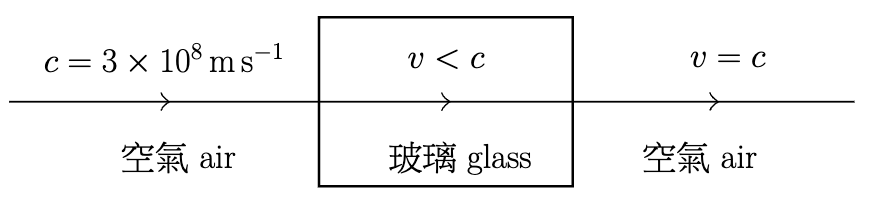
\includegraphics[width=0.666\linewidth]{assets/21389120782174281age.png}
        
        
    \end{figure}
\end{frame}

\begin{frame}{光的折射現象The phenomenon of the refraction of light}
    \begin{itemize}
        \item 當光從一種介質傳播到另一種具有不同速度的介質時,會發生\textbf{折射}。\\\textbf{Refraction} occurs when light travels from one medium to another medium with different speed.
        \item 因為不同介質有不同的速率,在以非零入射角進入另介質時光線會出現徧轉。\\Since light has different speeds in different mediums, light bends at a non-zero incident angle.
    \end{itemize}

\end{frame}




\begin{frame}{光的折射現象The phenomenon of the refraction of light}
\begin{itemize}
    \item 倘若光線通過界面時速率\textbf{變慢},折射線會\textbf{偏向法線}\\If light \textbf{loses speed} when crossing the boundary, it bends \textbf{towards the normal}.
\end{itemize}
    \begin{figure}
        \centering
        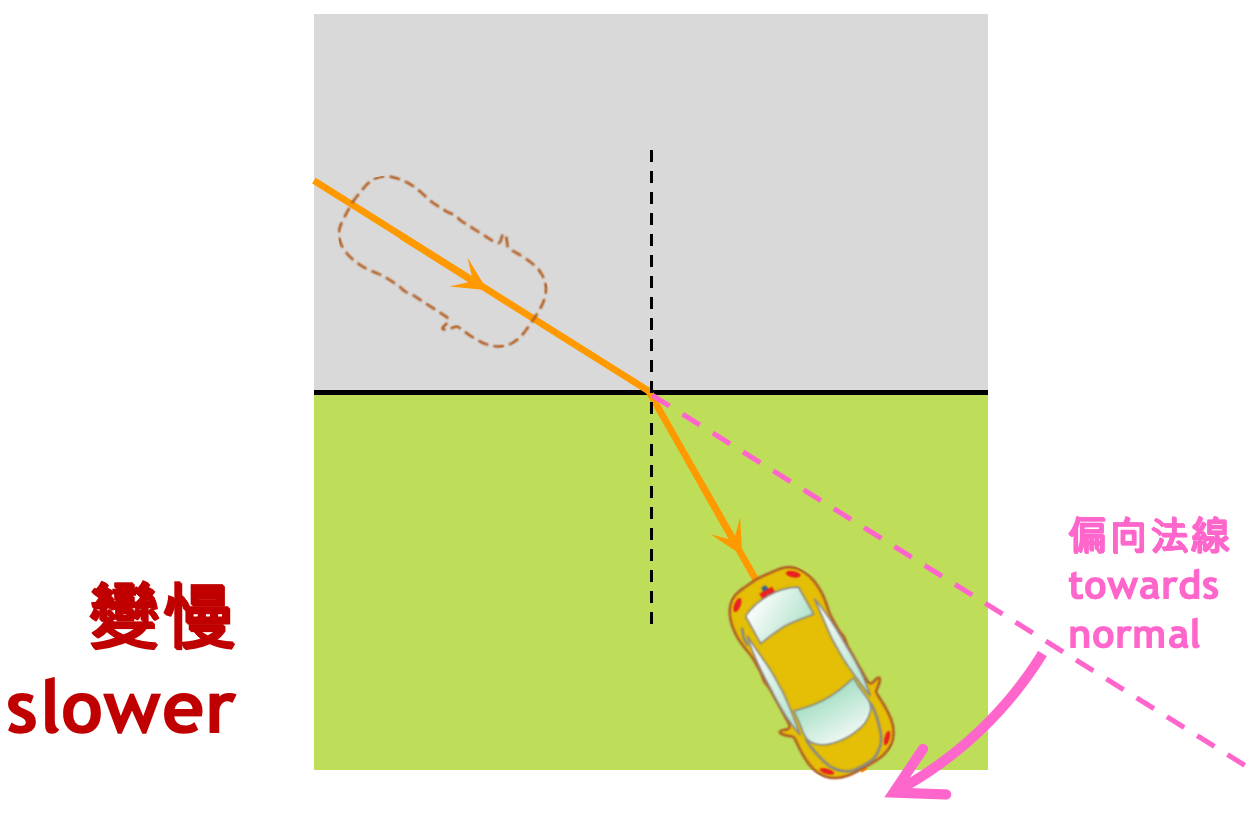
\includegraphics[width=.8\linewidth]{assets/123812904821.png}
    \end{figure}
\end{frame}
\begin{frame}{光的折射現象The phenomenon of the refraction of light}
\begin{itemize}
    \item 速率變得\textbf{愈慢},偏折程度\textbf{愈大}\\The \textbf{slower} it becomes, the \textbf{larger} it bends.
\end{itemize}
    \begin{figure}
        \centering
        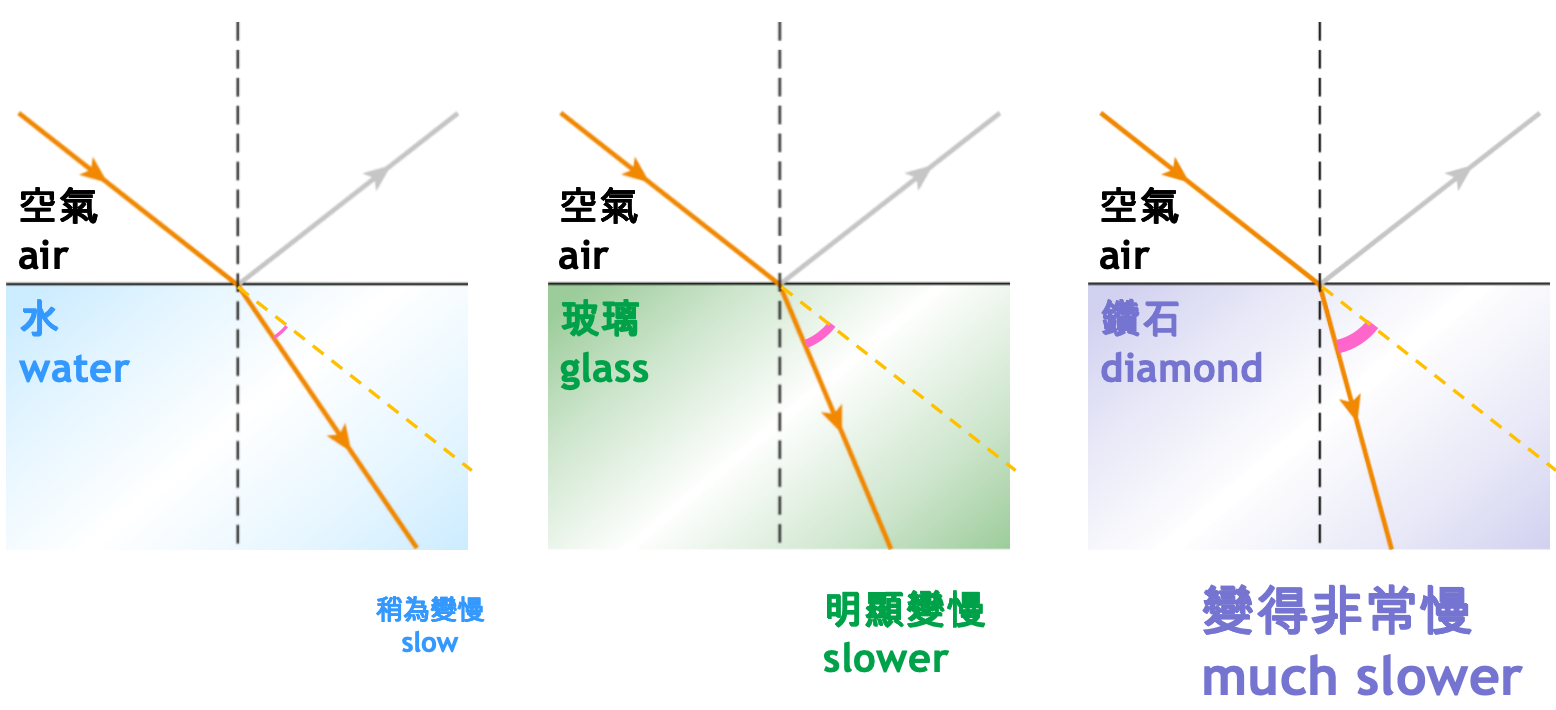
\includegraphics[width=1\linewidth]{assets/129380913812921.png}
    \end{figure}
\end{frame}

\begin{frame}{光的折射現象The phenomenon of the refraction of light}
\begin{itemize}
    \item 若光線的速率\textbf{變快},折射線會折射線會\textbf{偏離法線}\\if light \textbf{gains speed} at the boundary, it bends \textbf{away from the normal}.
\end{itemize}
    \begin{figure}
        \centering
        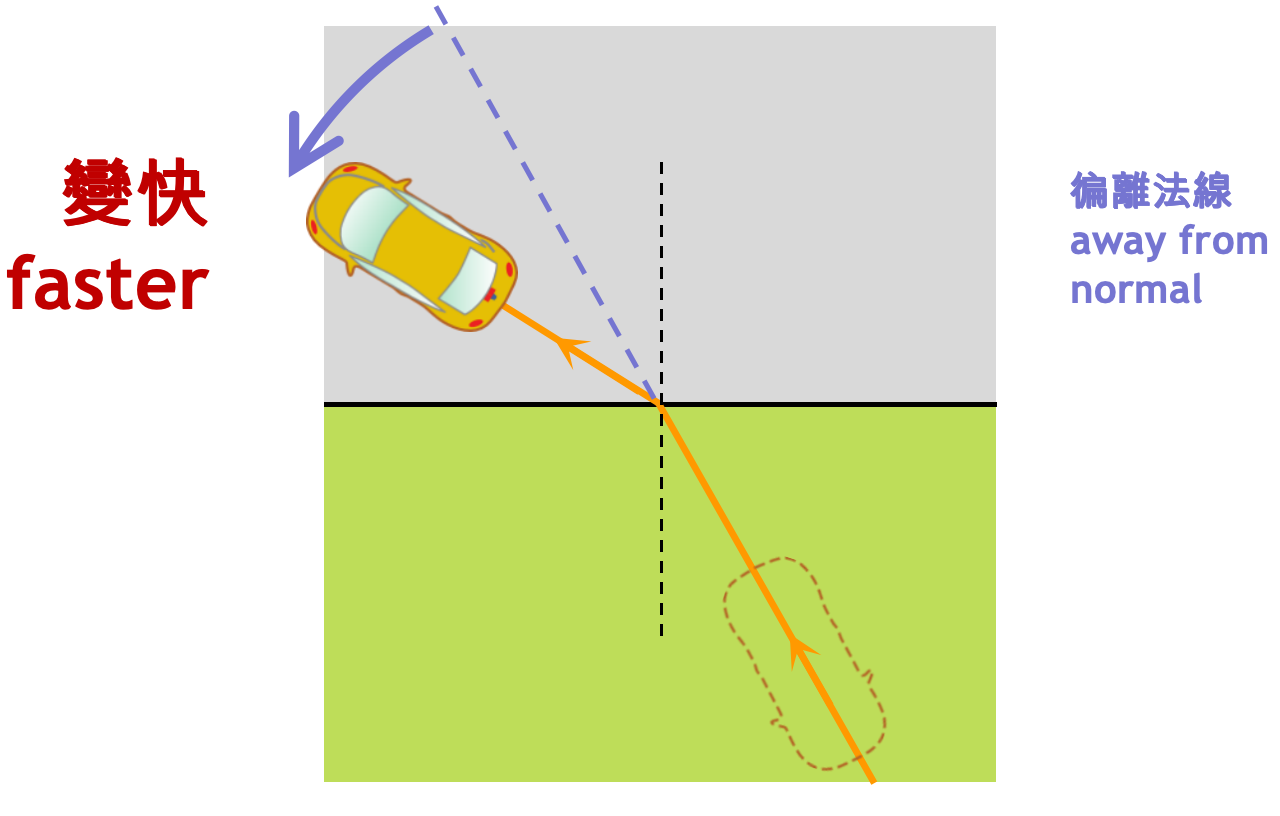
\includegraphics[width=.8\linewidth]{assets/3192803814912.png}
    \end{figure}
\end{frame}
\begin{frame}{光的折射現象The phenomenon of the refraction of light}
\begin{itemize}
    \item 速率變得\textbf{愈快},偏折程度\textbf{愈大}\\The \textbf{faster} it becomes, the \textbf{larger} it bends.
\end{itemize}
    \begin{figure}
        \centering
        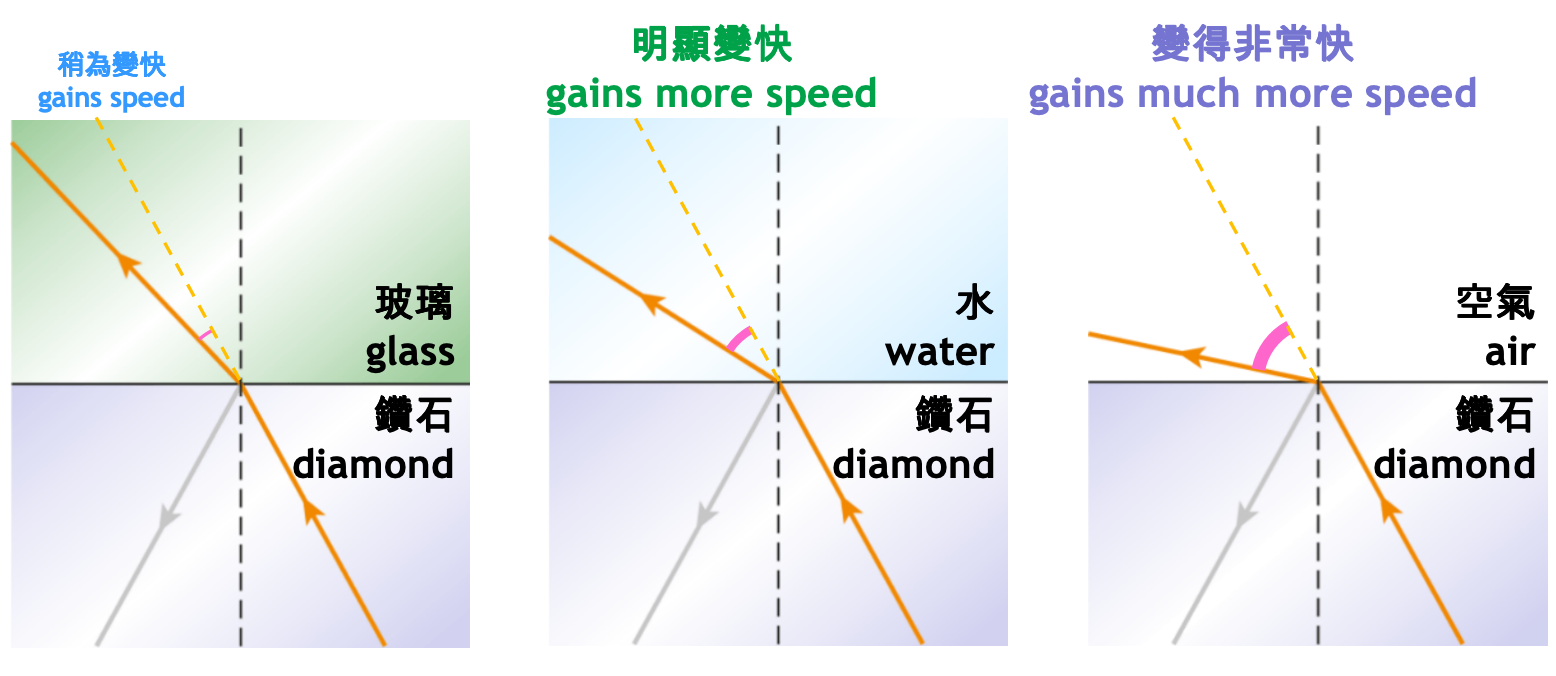
\includegraphics[width=1\linewidth]{assets/12803293age.png}
    \end{figure}
\end{frame}

\begin{frame}{折射定律 Law of Refraction}
    \begin{figure}
        \centering
        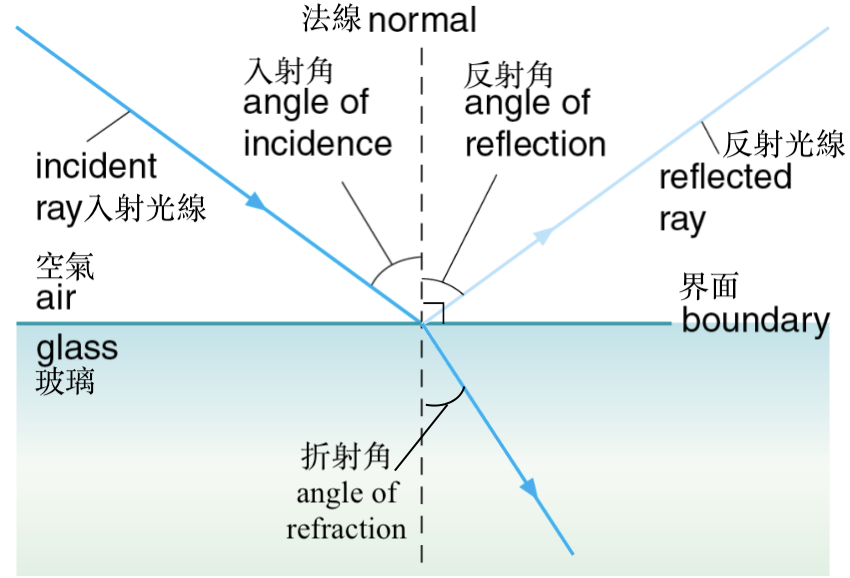
\includegraphics[width=0.75\linewidth]{assets/18309131294639.png}
        
        
    \end{figure}
\end{frame}
\begin{frame}{折射定律}
    \begin{figure}
        \centering
        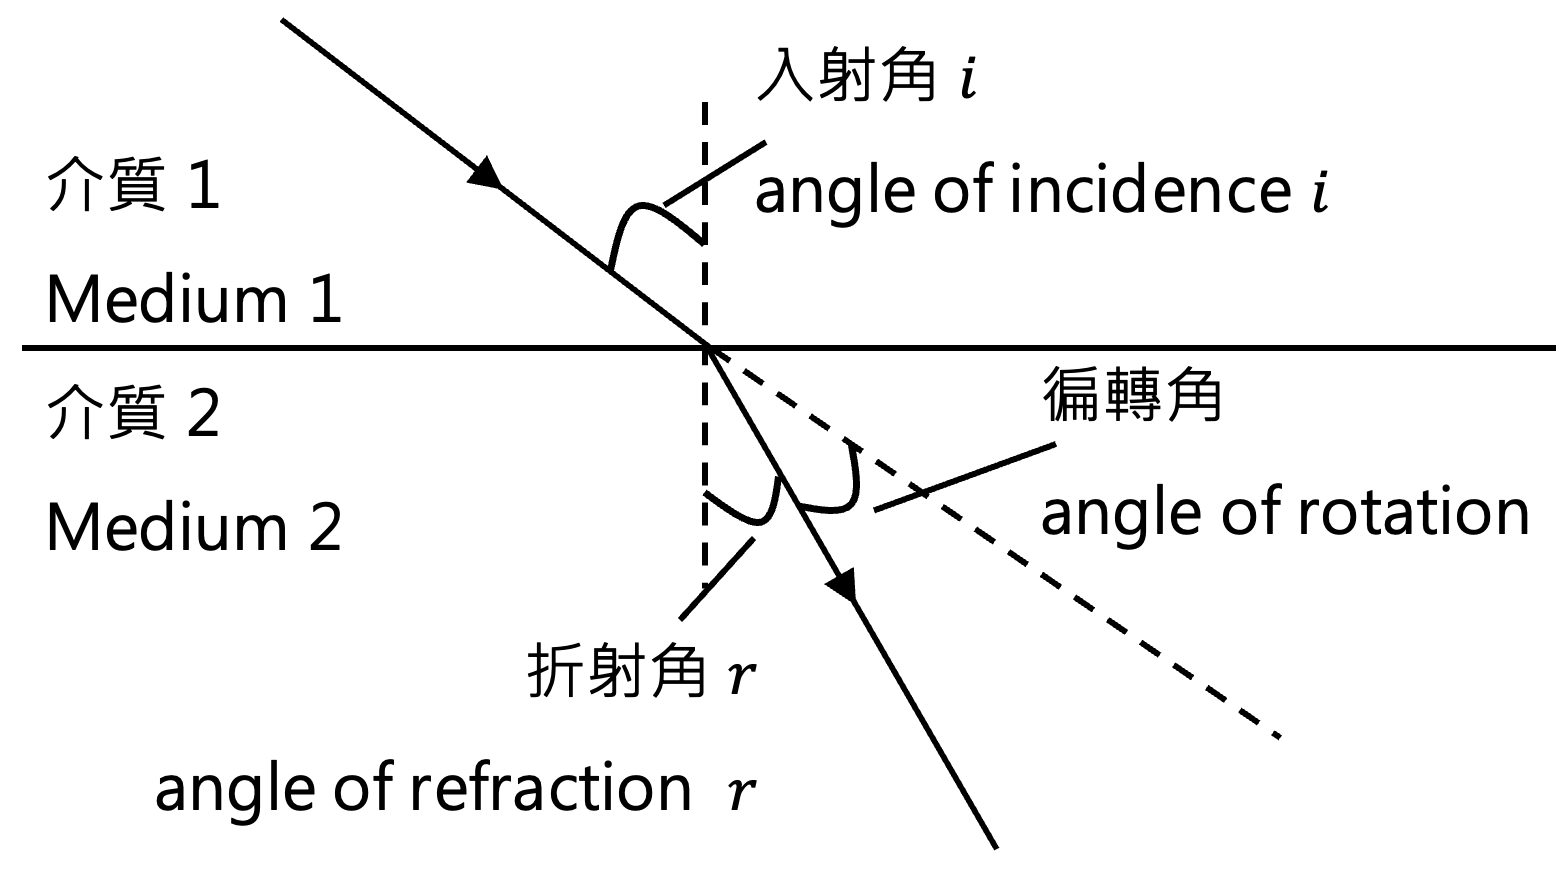
\includegraphics[width=1\linewidth]{assets/12903819232183921832.png}
        
        
    \end{figure}
\end{frame}

\begin{frame}{折射定律 Law of Refraction}
    \begin{alertblock}
        {折射定律 Law of Refraction}
            當光線從一個介質到另一個介質時,\\When a ray of light passes from one medium to another,\bigskip
        \begin{itemize}
        \setlength{\itemsep}{.8em}
            \item $\dfrac{\sin i}{\sin r}=$常數constant\medskip
            \begin{itemize}
                \item 亦稱為斯涅耳定律。\\also known as Snell's law.
            \end{itemize}
            \item 入射線、折射線和法線都去同一平面。\\the incident ray, the refracted ray and the normal all lie in the same plane.
        \end{itemize}

    \end{alertblock}
    
\end{frame}

\begin{eg}

    一束光從空氣射入一個半圓形的玻璃塊,入射角為 $i =$ \dg{45}。它在折射後的角度為 $r =$ \dg{30}。如果入射角為 $i =$ \dg{70},折射角為 $r =$?\\A ray of light is incident from air to a semicircular glass block with $i =$ \dg{45}. It is refracted at $r =$ \dg{30}. If $i =$ \dg{70}, $r =$ ?
    \begin{columns}

        \column{.5\textwidth}
        \column{.5\textwidth}
        \begin{figure}
            \centering
            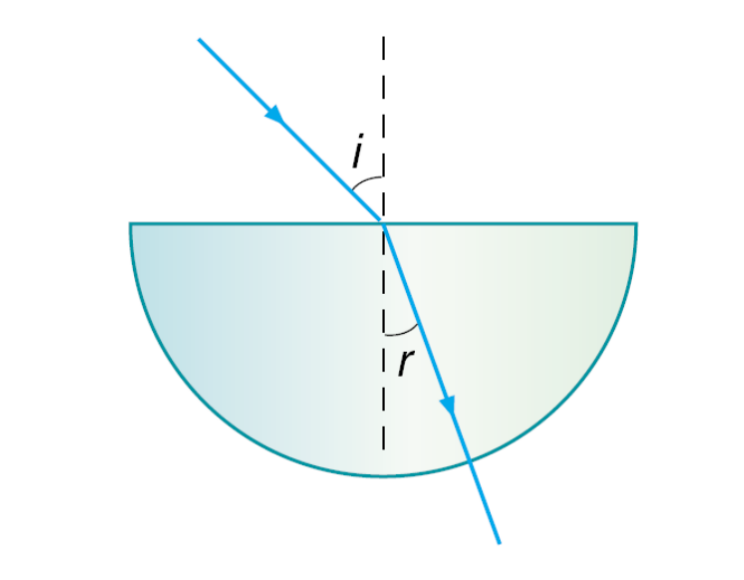
\includegraphics[width=1\linewidth]{assets/218129849734.png}
            
            
        \end{figure}
    \end{columns}
\end{eg}

\begin{frame}{折射率Refractive index}
    \begin{exampleblock}
        {某介質的折射率 n \\The refractive index of a medium n}
        \begin{align*}
            n=\frac{c}{v}
        \end{align*}
    \end{exampleblock}
    \begin{itemize}
        \item v - 光線在介質內的速率。\\v - speed of light in medium
        \item c - 光線在真空/空氣速率。($=$ \vel{3e8})\\c -  speed of light in vacuum or air. ($=$ \vel{3e8})
        \item n沒有單位。 \\n has no units.
    \end{itemize}
\end{frame}


\begin{frame}{折射率Refractive index}
    \begin{itemize}
   
        \item n越大,光線徧折程度更大\\n larger, light ray bends more
        \item \textbf{光密介質}:\textbf{Optically denser medium}:
        \begin{itemize}
            \item 介質有較大的n。medium with greater n
        \end{itemize}
        \item \textbf{光疏介質}\\\textbf{Optically less dense medium}:
        \begin{itemize}
            \item 介質有較小的n。medium with smaller n
        \end{itemize}
    \end{itemize}
\begin{figure}
    \centering
    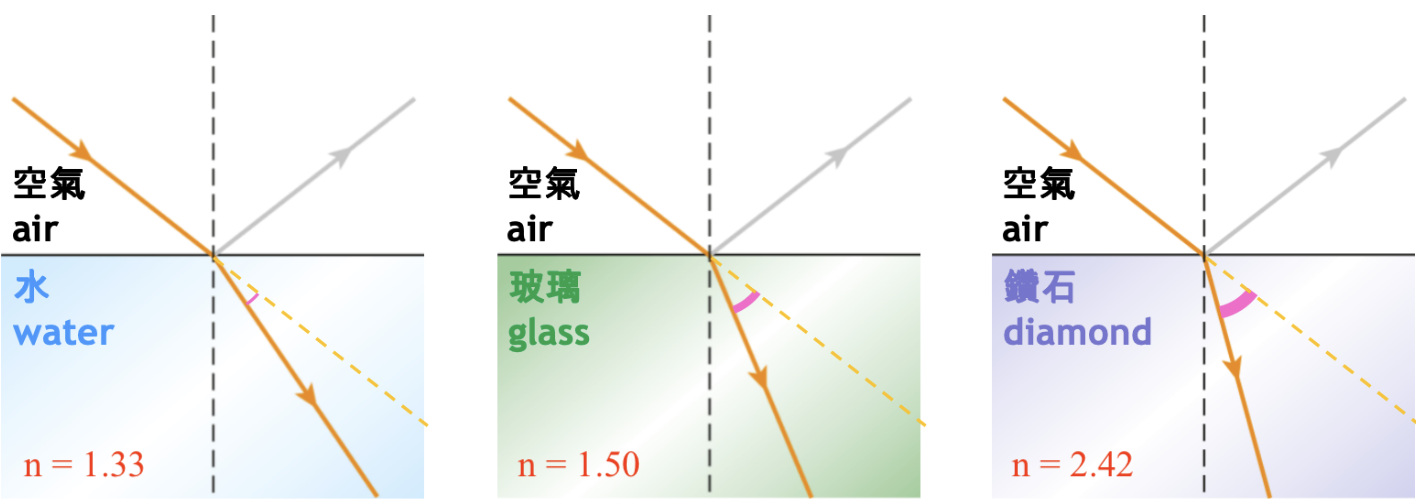
\includegraphics[width=0.75\linewidth]{assets/qdwqdij1342432.png}
\end{figure}
\end{frame}


\begin{frame}{不同介質的折射率 Some typical values of n}
    \begin{figure}
        \centering
        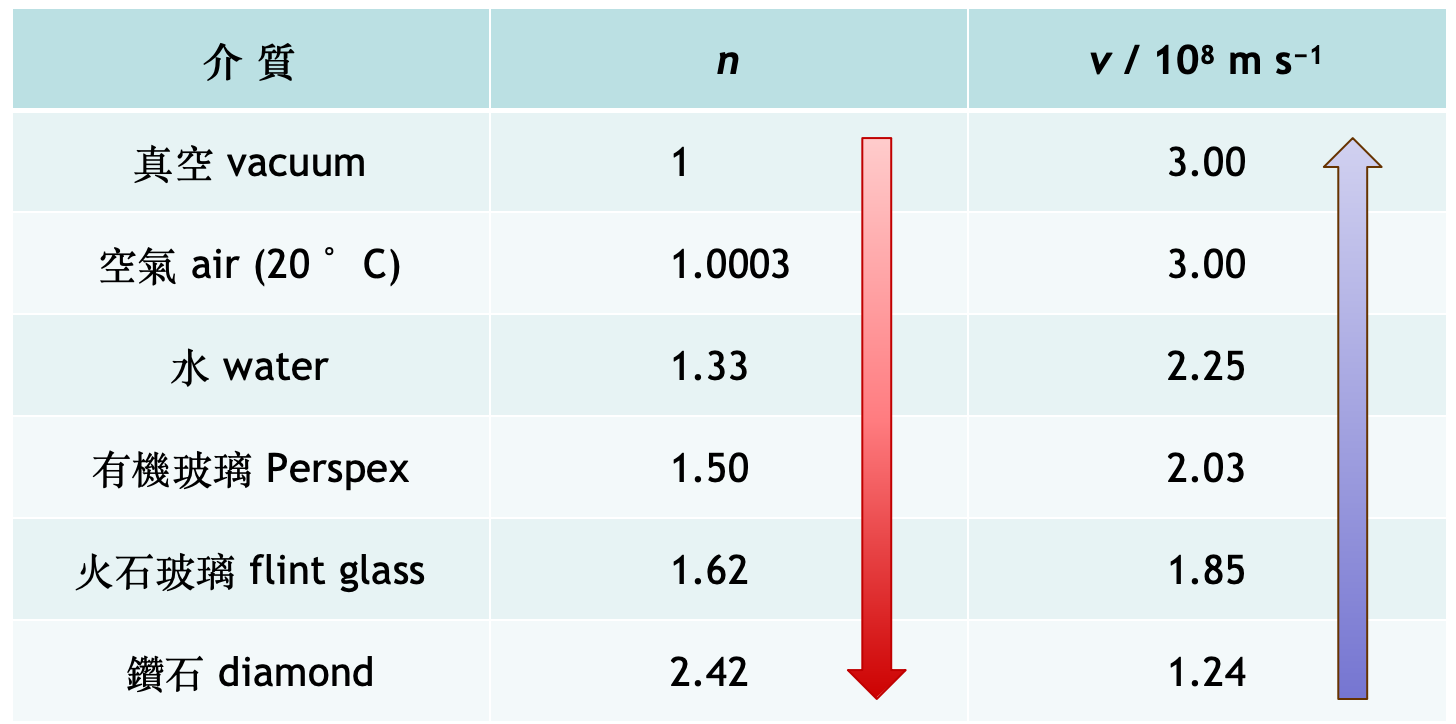
\includegraphics[width=0.9\linewidth]{assets/1290831em1.png}
        
        
    \end{figure}
\end{frame}



\begin{frame}{重溫斯涅耳定律Revision on Snell's law}
    \begin{alertblock}
        {斯涅耳定律Snell's law}
        \begin{align*}
            \frac{\sin\theta_1}{\sin \theta_2}=\frac{n_2}{n_1}=\frac{v_1}{v_2}
        \end{align*}
    \end{alertblock}
    換言之 in other words, $\sin\theta\propto v\propto \frac{1}{n}$
    \begin{figure}
        \centering
        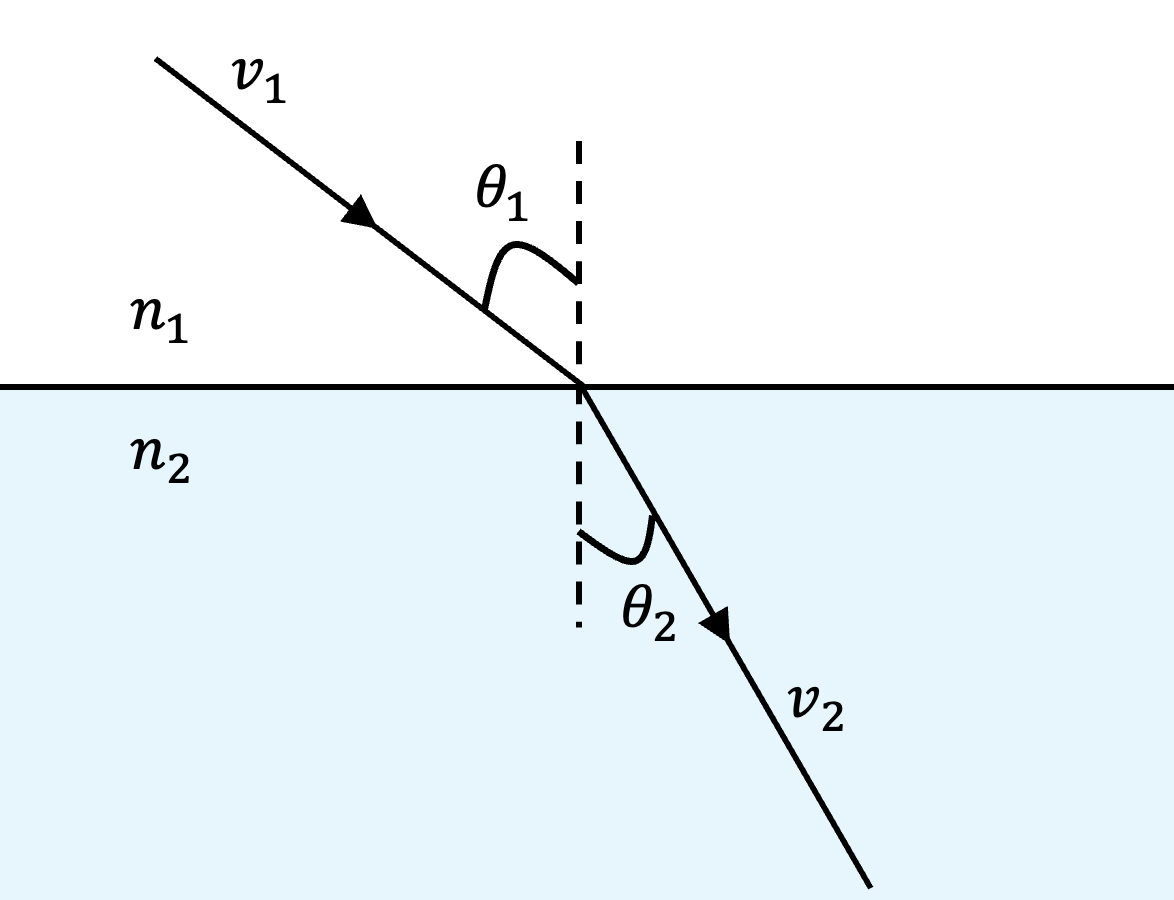
\includegraphics[width=0.5\linewidth]{assets/2109si91292.png}
    \end{figure}
\end{frame}

\begin{eg}
    \begin{figure}
        \centering
        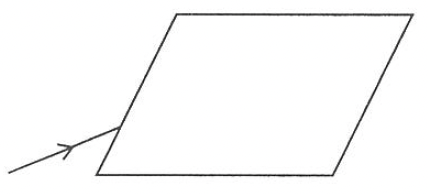
\includegraphics[width=0.5\linewidth]{assets/92180931283128.png}
    \end{figure}
    光線在空氣中傳播並穿透玻璃塊,如上所示。以下哪個圖示最能展示光線的路徑?\\A ray of light travels in air and strikes a glass block as shown above. Which of the following diagrams best shows the path of the ray?
\end{eg}

\begin{eg}
    \begin{tasks}(2)
        \task \topalign{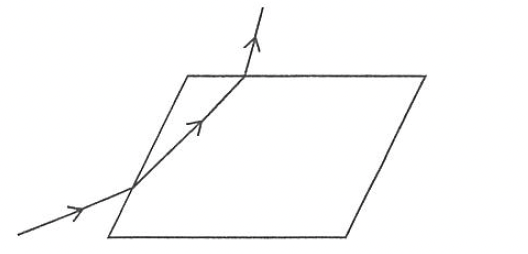
\includegraphics[width=.85\linewidth]{assets/du8u892j83892.png}}
        \task\topalign{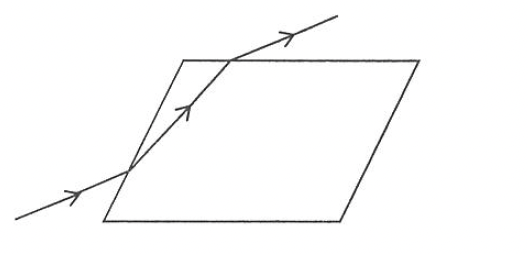
\includegraphics[width=0.85\linewidth]{assets/qeqeuj98ue823ue829un3e32.png}}
    \task\topalign{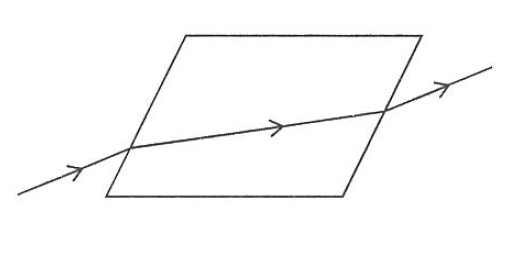
\includegraphics[width=0.85\linewidth]{assets/qqweqwwd39di30.png}}
    \task\topalign{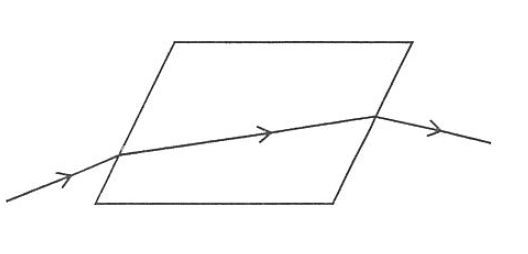
\includegraphics[width=0.85\linewidth]{assets/eqee32e23e23e2e3.png}}
    \end{tasks}
\end{eg}

\begin{eg}
圖中是一束從介質I到介質III的光線的路徑。請按照折射率和光在各介質中的速率降序排列。\\The figure shows the path of a light ray travelling from medium I to medium III separated by parallel boundaries. Arrange in descending order the refractive index and speed of light in the respective media.
    \begin{figure}
        \centering
        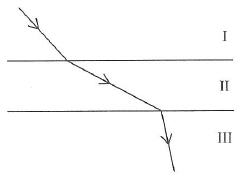
\includegraphics[width=0.5\linewidth]{assets/8eu89c2n28.png}
    \end{figure}
\end{eg}


\begin{eg}
    圖中所示為一條光線通過一個塑膠製的三稜鏡的路徑。光線以角度\dg{50}射向稜鏡的邊PQ。\\A ray of light passes through a triangular plastic prism as shown. The ray strikes the side PQ at an angle of \dg{50}.
    \begin{figure}
        \centering
        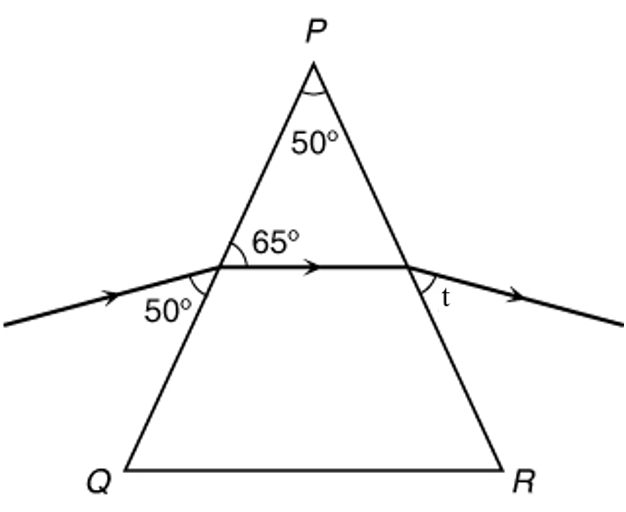
\includegraphics[width=0.5\linewidth]{assets/9209138209312.png}
        
        
    \end{figure}
    
\end{eg}

\begin{eg}
    \begin{itemize}
        \item [(a)] 求該塑膠的折射率和$t$。\\Find the refractive index of the plastic and $t$.
    \end{itemize}
\end{eg}

\begin{eg}
    \begin{itemize}
        \item [(b)] 假設光線以角度\dg{60}射向邊PQ,繪畫光線通過稜鏡的路徑。\\Suppose the light ray strikes the side PQ at angle of \dg{60}. Sketch the path of the light ray travelling through and out of the prism.
    \end{itemize}
    \begin{figure}
        \centering
        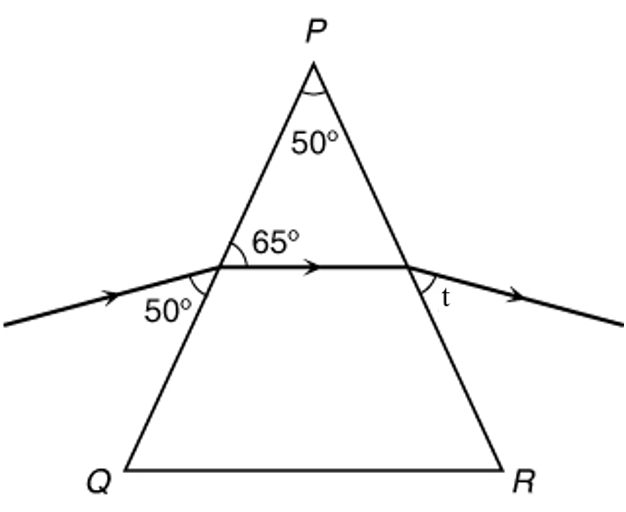
\includegraphics[width=0.6\linewidth]{assets/9209138209312.png}
        
        
    \end{figure}
\end{eg}

\begin{eg}
    \begin{figure}
        \centering
        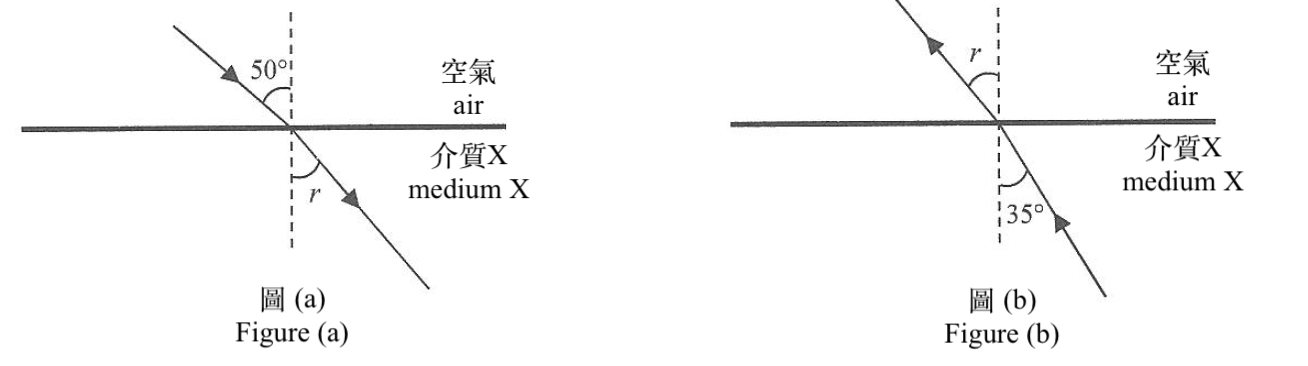
\includegraphics[width=1\linewidth]{assets/212109281938.png}
    \end{figure}
    圖(a)顯示了一束光線從空氣進入介質$X$。入射角為\dg{50},折射角為$r$。另一束從介質$X$進入空氣的光線顯示在圖(b)中。入射角為\dg{35},折射角也等於$r$。求r。\\Figure (a) shows a light ray travelling from air into medium $X$. The angle of incidence is \dg{50} and the angle of refraction is $r$. Another light ray travelling from medium $X$ to air is shown in Figure (b). The angle of incidence is \dg{35} and the angle of refraction is also equal to $r$. What is angle $r$?
\end{eg}

\begin{eg}
    \begin{itemize}
        \item [sol.]
    \end{itemize}
\end{eg}


\begin{frame}{色散Dispersion}
    \begin{itemize}
        \item 白光由多種顏色混合而成。\\White light is composed of a mixture of colors.
        \item 當光線通過一個棱鏡時,會發生兩次折射,並將光線分離成不同的顏色。\\When light passes through a prism, it is refracted twice and separated into different colors.
    \end{itemize}
    \begin{figure}
        \centering
        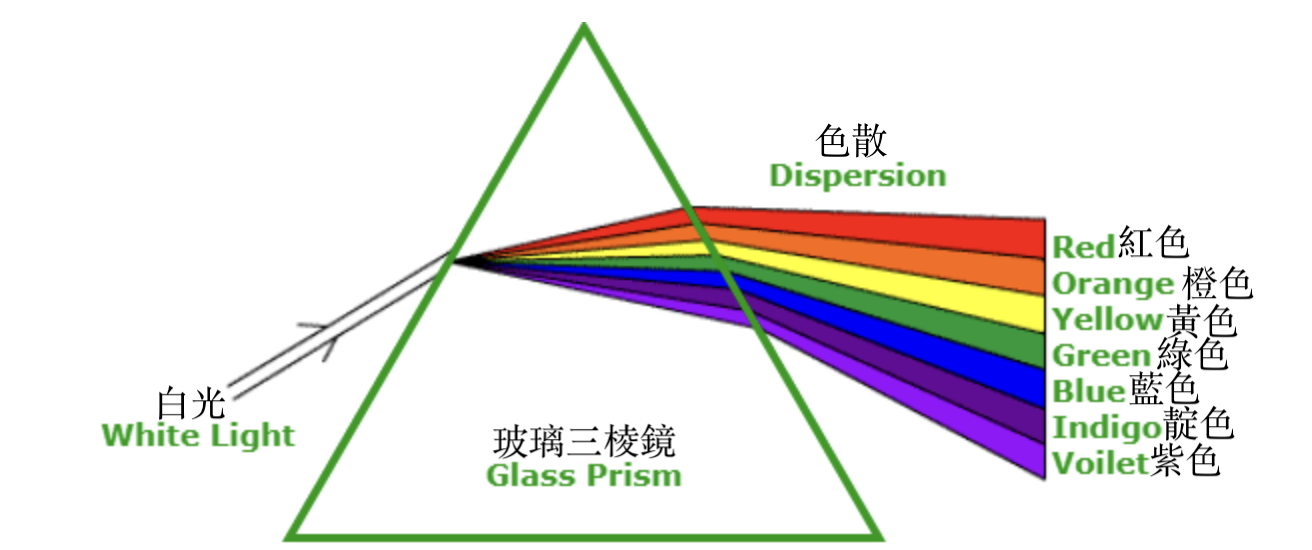
\includegraphics[width=0.75\linewidth]{assets/qdwdqdwq1111e.png}
    \end{figure}
\end{frame}

\begin{frame}{色散Dispersion}
    \begin{itemize}
        \item 玻璃中光的速度$v$和每種顏色的折射率$n$是不同的。\\The speed of light $v$ in glass and the refractive index $n$ of glass for each color are different.
        \item 在玻璃中對於可見光來說,紅光具有最低的折射率$n$,而紫光具有最高的折射率$n$。\\In glass and for visible light, red light has the lowest $n$ and violet light has the highest $n$.
    \end{itemize}
    \begin{figure}
        \centering
        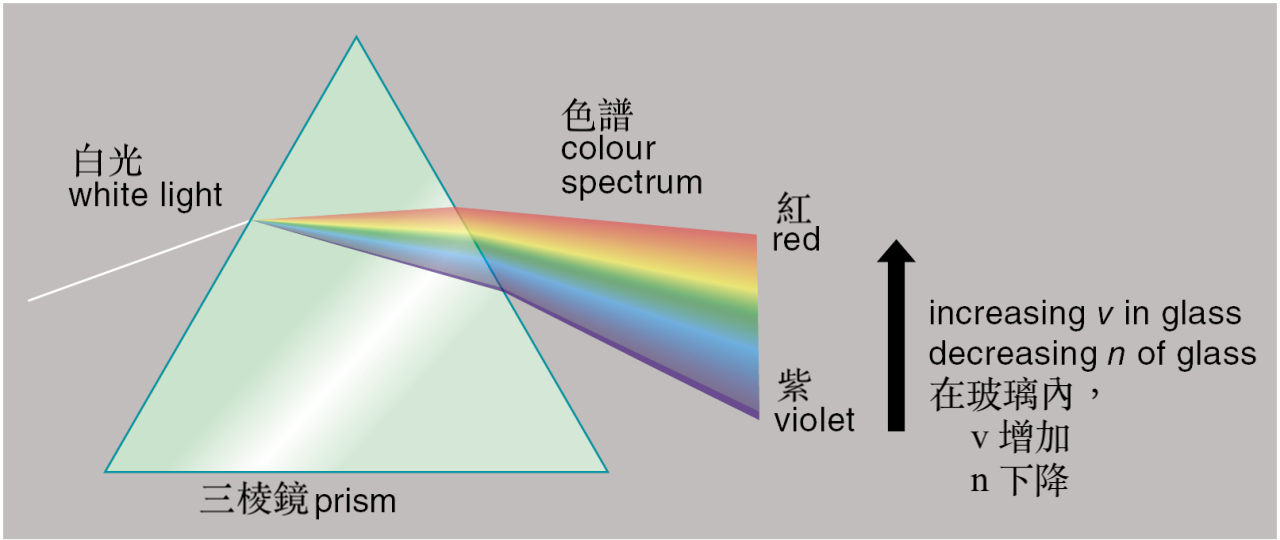
\includegraphics[width=0.75\linewidth]{assets/ddqwdqwdwq1111ge.png}
        
        
    \end{figure}
\end{frame}
\begin{frame}{色散Dispersion}
    \begin{itemize}
        \item 在玻璃中對於可見光來說,紅光具有最低的折射率$n$,而紫光具有最高的折射率$n$。\\In glass and for visible light, red light has the lowest $n$ and violet light has the highest $n$.
        
    \end{itemize}
    \begin{figure}
        \centering
        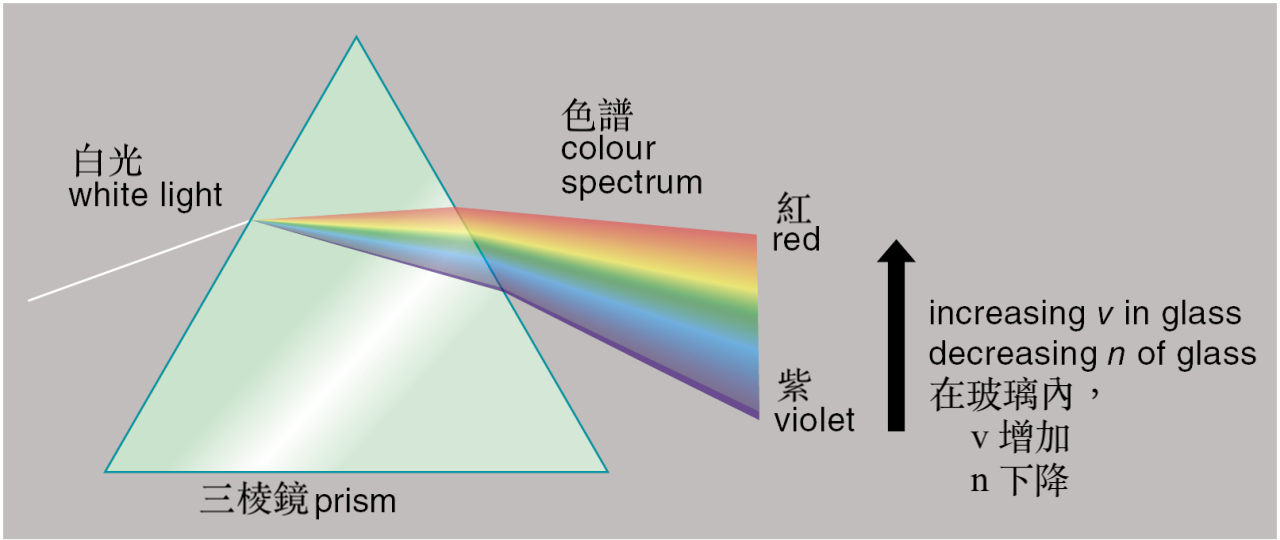
\includegraphics[width=0.75\linewidth]{assets/ddqwdqwdwq1111ge.png}
        
        
    \end{figure}
\end{frame}

\begin{frame}{色散Dispersion}
    \begin{itemize}
        \item 紫光在從空氣到玻璃,或從玻璃到空氣時徧折的程度比紅光更大。\\Violet light bends more than red light when going from air to glass, or glass to air.
    \end{itemize}\bigskip
    \begin{figure}
        \centering
        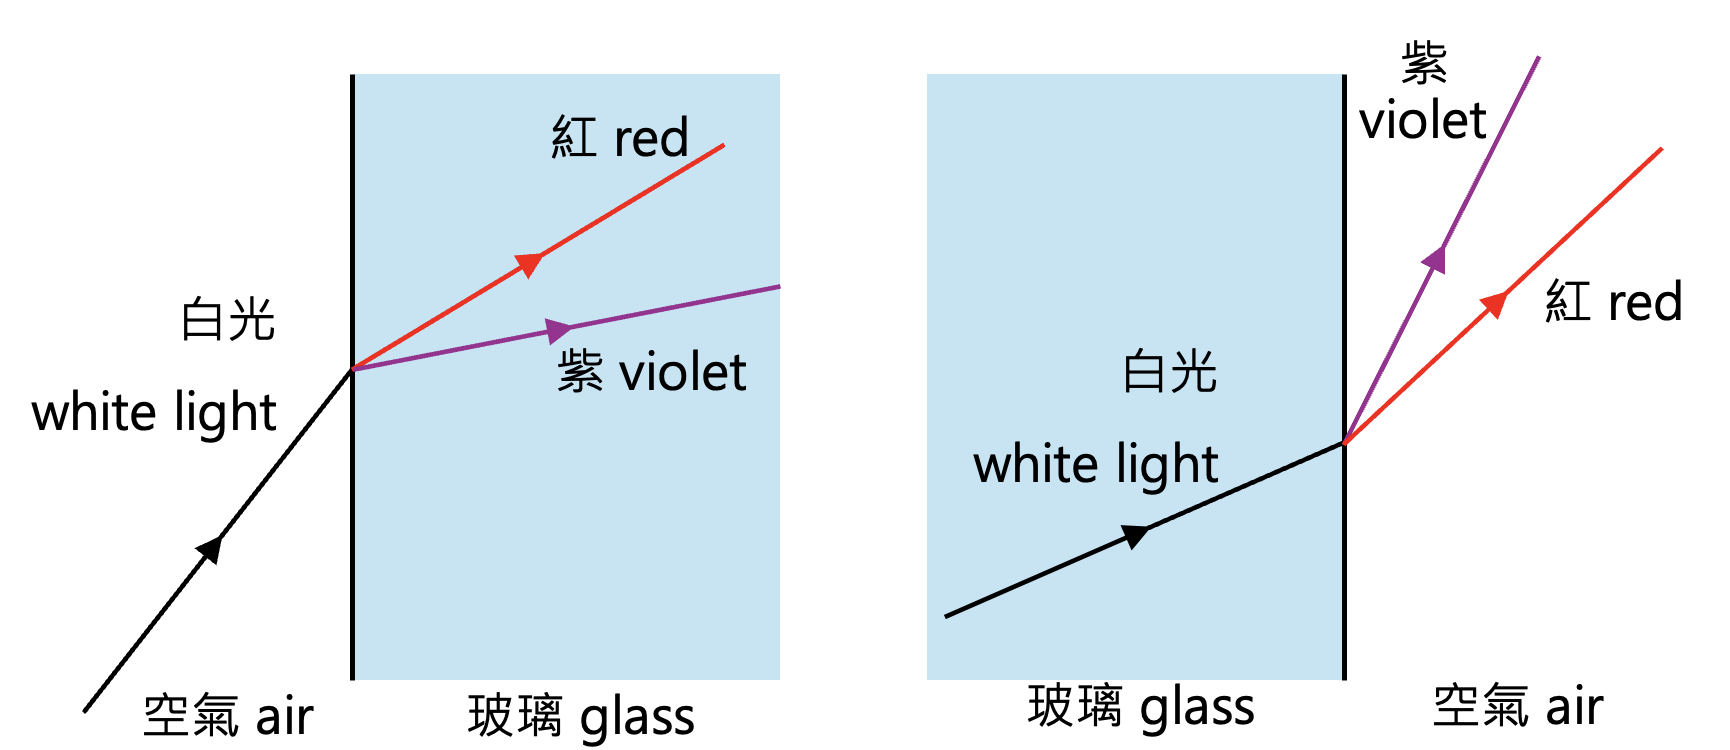
\includegraphics[width=0.85\linewidth]{assets/8un981xue1.png}
    \end{figure}
\end{frame}

\begin{frame}{}
    
\end{frame}

\begin{eg}
    考慮一個玻璃三棱鏡ABC,一束白光以入射角\dg{60}入射到AB面上。求在AC面上紅光和紫光的折射角。己知玻璃的折射率,對於紫光為1.665,對於紅光為1.618。\\Consider a regular glass prism ABC, a white light is incident on surface AB with incident angle \dg{60}. Find the angle of refraction for red and violet rays at side AC. The index of refraction of glass violet light is 1.665 and for red light 1.618.
    \begin{figure}
        \centering
        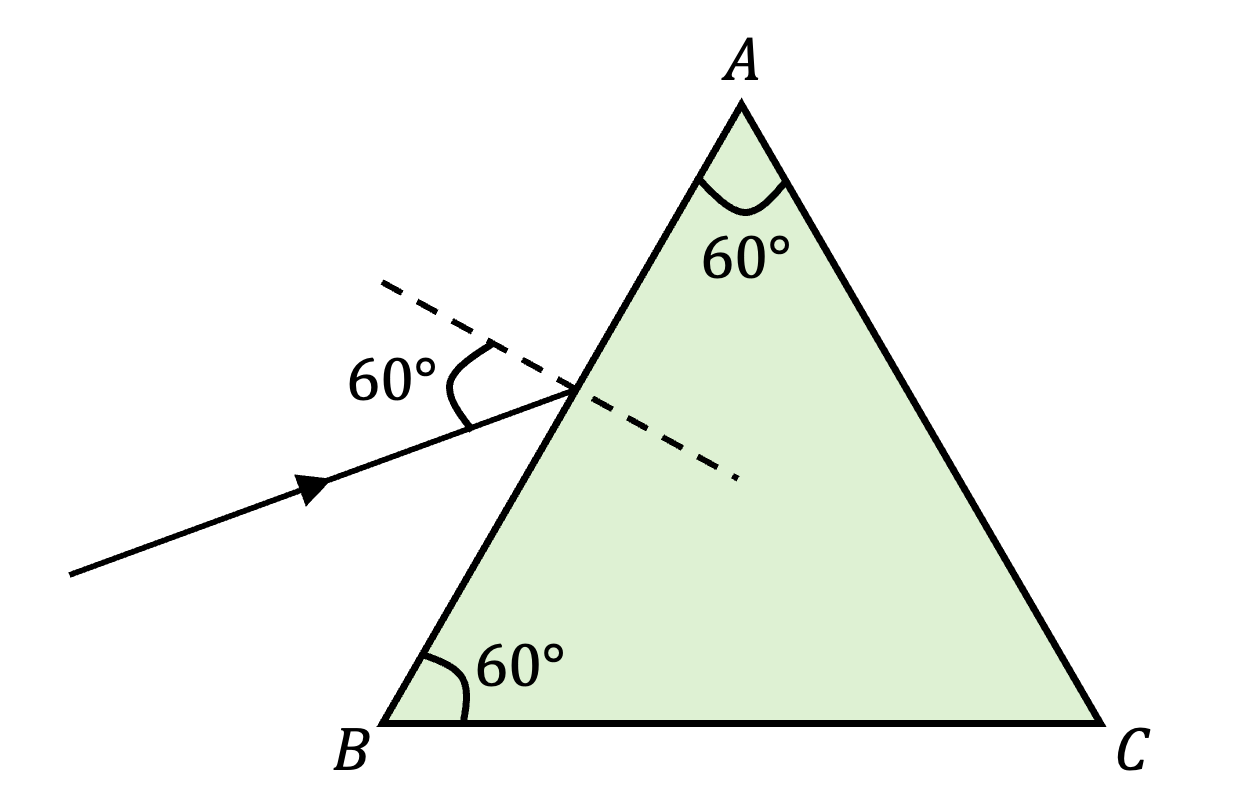
\includegraphics[width=0.5\linewidth]{assets/dedwed2232321312.png}
    \end{figure}
\end{eg}



















































































\end{document}